\subsection{Task 5.2: Potentially shareable non-shared trips}
To estimate how many non-shared trips may have had a plausible sharing partner, we screen Uber and Lyft $N/N$ trips using a transparent zone-time rule. A trip is counted as potentially shareable if at least one other $N/N$ trip from the same platform and pickup month has the same directed OD pair and falls in the same pickup-time window. The main specification uses a 10-minute pickup window; 5- and 15-minute windows are reported as sensitivity checks. Completed trips must have official pickup/dropoff zones and $0<\mathrm{trip\_miles}\leq100$.
\begin{table}[htbp]\centering\small\caption{Task 5.2 potential shareability under the same-OD, 10-minute pickup-window rule.}\label{tab:t5potential}\begin{tabular}{llrrrr}\hline Month & Platform & Eligible $N/N$ & Potentially shareable & Share & Candidate pairs \\ \hline
2026-04 & Uber & 14,958,704 & 6,790,245 & 45.4\% & 9,356,742 \\
2026-04 & Lyft & 5,613,764 & 1,497,505 & 26.7\% & 1,361,286 \\
2026-05 & Uber & 14,962,744 & 6,701,182 & 44.8\% & 9,060,008 \\
2026-05 & Lyft & 6,766,606 & 1,915,041 & 28.3\% & 1,812,575 \\
\hline\end{tabular}\end{table}
\begin{figure}[htbp]\centering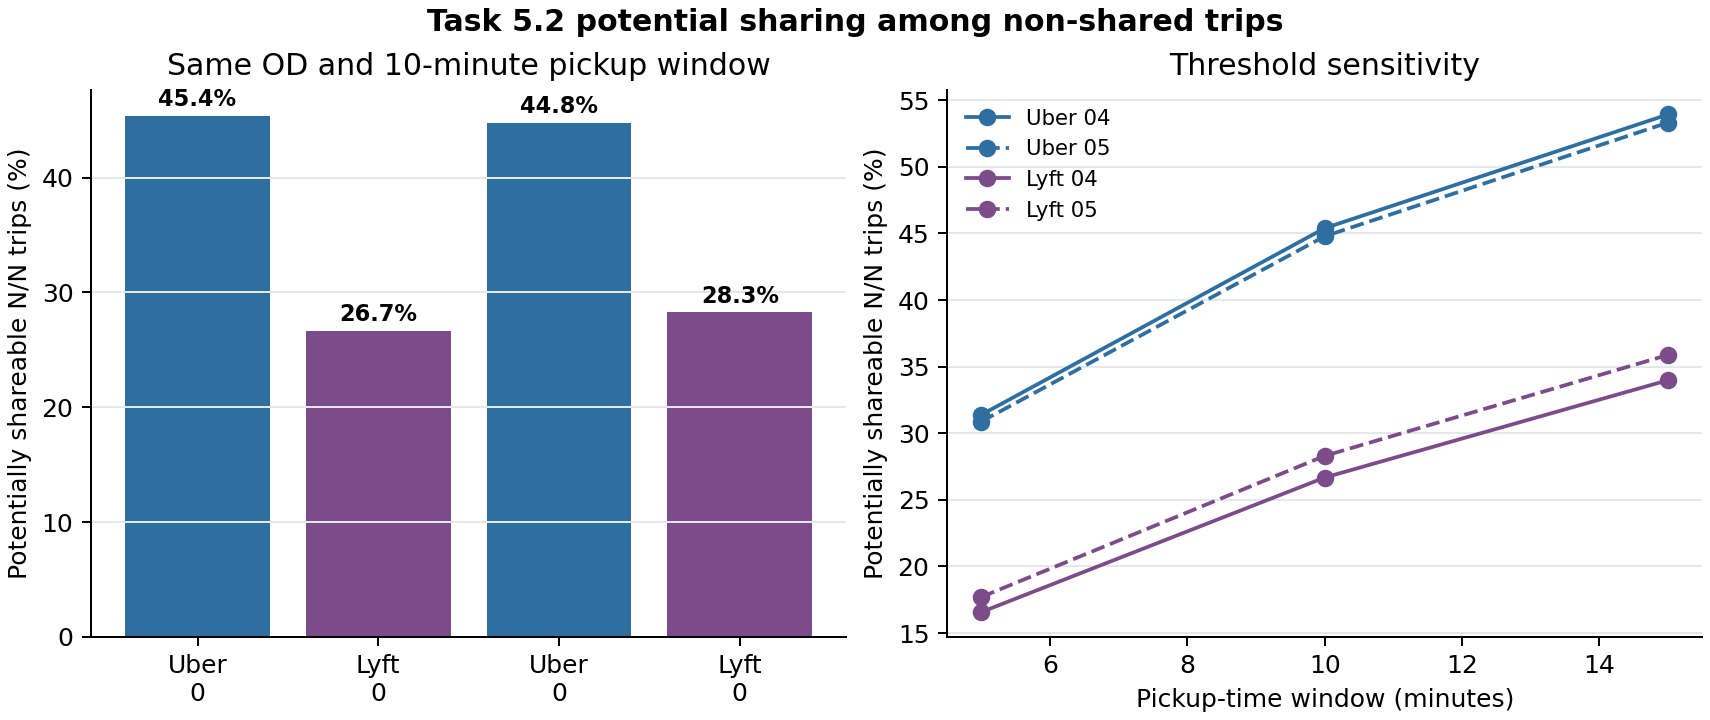
\includegraphics[width=.82\textwidth]{04_Results/Task_5/figures/potential_sharing.png}\caption{Potentially shareable non-shared trips under same-OD pickup-window rules. The left panel reports the 10-minute main rule; the right panel shows sensitivity to 5-, 10-, and 15-minute windows.}\label{fig:t5potential}\end{figure}
This screen suggests that a substantial share of non-shared completed trips had at least one coarse zone-time neighbor. Under the 10-minute rule, Uber has about 45.4\% in April and 44.8\% in May; Lyft has about 26.7\% and 28.3\%. The sensitivity table shows the expected monotonic pattern: wider pickup windows increase the potential-shareable count. These values should not be interpreted as trips that definitely could be pooled. Taxi Zones hide exact endpoints, the rule does not model waiting tolerance, detour cost, vehicle capacity, dispatch feasibility, or passenger willingness, and trips close to a time-window boundary may be misclassified. The result is therefore an upper-screening measure of latent co-occurrence in the non-shared trip stream, not a platform matching rate.
